% Options for packages loaded elsewhere
\PassOptionsToPackage{unicode}{hyperref}
\PassOptionsToPackage{hyphens}{url}
%
\documentclass[
]{article}
\usepackage{amsmath,amssymb}
\usepackage{lmodern}
\usepackage{ifxetex,ifluatex}
\ifnum 0\ifxetex 1\fi\ifluatex 1\fi=0 % if pdftex
  \usepackage[T1]{fontenc}
  \usepackage[utf8]{inputenc}
  \usepackage{textcomp} % provide euro and other symbols
\else % if luatex or xetex
  \usepackage{unicode-math}
  \defaultfontfeatures{Scale=MatchLowercase}
  \defaultfontfeatures[\rmfamily]{Ligatures=TeX,Scale=1}
\fi
% Use upquote if available, for straight quotes in verbatim environments
\IfFileExists{upquote.sty}{\usepackage{upquote}}{}
\IfFileExists{microtype.sty}{% use microtype if available
  \usepackage[]{microtype}
  \UseMicrotypeSet[protrusion]{basicmath} % disable protrusion for tt fonts
}{}
\makeatletter
\@ifundefined{KOMAClassName}{% if non-KOMA class
  \IfFileExists{parskip.sty}{%
    \usepackage{parskip}
  }{% else
    \setlength{\parindent}{0pt}
    \setlength{\parskip}{6pt plus 2pt minus 1pt}}
}{% if KOMA class
  \KOMAoptions{parskip=half}}
\makeatother
\usepackage{xcolor}
\IfFileExists{xurl.sty}{\usepackage{xurl}}{} % add URL line breaks if available
\IfFileExists{bookmark.sty}{\usepackage{bookmark}}{\usepackage{hyperref}}
\hypersetup{
  pdftitle={Lab 1: exponential growth},
  pdfauthor={NRES 470/670},
  hidelinks,
  pdfcreator={LaTeX via pandoc}}
\urlstyle{same} % disable monospaced font for URLs
\usepackage[margin=1in]{geometry}
\usepackage{color}
\usepackage{fancyvrb}
\newcommand{\VerbBar}{|}
\newcommand{\VERB}{\Verb[commandchars=\\\{\}]}
\DefineVerbatimEnvironment{Highlighting}{Verbatim}{commandchars=\\\{\}}
% Add ',fontsize=\small' for more characters per line
\usepackage{framed}
\definecolor{shadecolor}{RGB}{248,248,248}
\newenvironment{Shaded}{\begin{snugshade}}{\end{snugshade}}
\newcommand{\AlertTok}[1]{\textcolor[rgb]{0.94,0.16,0.16}{#1}}
\newcommand{\AnnotationTok}[1]{\textcolor[rgb]{0.56,0.35,0.01}{\textbf{\textit{#1}}}}
\newcommand{\AttributeTok}[1]{\textcolor[rgb]{0.77,0.63,0.00}{#1}}
\newcommand{\BaseNTok}[1]{\textcolor[rgb]{0.00,0.00,0.81}{#1}}
\newcommand{\BuiltInTok}[1]{#1}
\newcommand{\CharTok}[1]{\textcolor[rgb]{0.31,0.60,0.02}{#1}}
\newcommand{\CommentTok}[1]{\textcolor[rgb]{0.56,0.35,0.01}{\textit{#1}}}
\newcommand{\CommentVarTok}[1]{\textcolor[rgb]{0.56,0.35,0.01}{\textbf{\textit{#1}}}}
\newcommand{\ConstantTok}[1]{\textcolor[rgb]{0.00,0.00,0.00}{#1}}
\newcommand{\ControlFlowTok}[1]{\textcolor[rgb]{0.13,0.29,0.53}{\textbf{#1}}}
\newcommand{\DataTypeTok}[1]{\textcolor[rgb]{0.13,0.29,0.53}{#1}}
\newcommand{\DecValTok}[1]{\textcolor[rgb]{0.00,0.00,0.81}{#1}}
\newcommand{\DocumentationTok}[1]{\textcolor[rgb]{0.56,0.35,0.01}{\textbf{\textit{#1}}}}
\newcommand{\ErrorTok}[1]{\textcolor[rgb]{0.64,0.00,0.00}{\textbf{#1}}}
\newcommand{\ExtensionTok}[1]{#1}
\newcommand{\FloatTok}[1]{\textcolor[rgb]{0.00,0.00,0.81}{#1}}
\newcommand{\FunctionTok}[1]{\textcolor[rgb]{0.00,0.00,0.00}{#1}}
\newcommand{\ImportTok}[1]{#1}
\newcommand{\InformationTok}[1]{\textcolor[rgb]{0.56,0.35,0.01}{\textbf{\textit{#1}}}}
\newcommand{\KeywordTok}[1]{\textcolor[rgb]{0.13,0.29,0.53}{\textbf{#1}}}
\newcommand{\NormalTok}[1]{#1}
\newcommand{\OperatorTok}[1]{\textcolor[rgb]{0.81,0.36,0.00}{\textbf{#1}}}
\newcommand{\OtherTok}[1]{\textcolor[rgb]{0.56,0.35,0.01}{#1}}
\newcommand{\PreprocessorTok}[1]{\textcolor[rgb]{0.56,0.35,0.01}{\textit{#1}}}
\newcommand{\RegionMarkerTok}[1]{#1}
\newcommand{\SpecialCharTok}[1]{\textcolor[rgb]{0.00,0.00,0.00}{#1}}
\newcommand{\SpecialStringTok}[1]{\textcolor[rgb]{0.31,0.60,0.02}{#1}}
\newcommand{\StringTok}[1]{\textcolor[rgb]{0.31,0.60,0.02}{#1}}
\newcommand{\VariableTok}[1]{\textcolor[rgb]{0.00,0.00,0.00}{#1}}
\newcommand{\VerbatimStringTok}[1]{\textcolor[rgb]{0.31,0.60,0.02}{#1}}
\newcommand{\WarningTok}[1]{\textcolor[rgb]{0.56,0.35,0.01}{\textbf{\textit{#1}}}}
\usepackage{graphicx}
\makeatletter
\def\maxwidth{\ifdim\Gin@nat@width>\linewidth\linewidth\else\Gin@nat@width\fi}
\def\maxheight{\ifdim\Gin@nat@height>\textheight\textheight\else\Gin@nat@height\fi}
\makeatother
% Scale images if necessary, so that they will not overflow the page
% margins by default, and it is still possible to overwrite the defaults
% using explicit options in \includegraphics[width, height, ...]{}
\setkeys{Gin}{width=\maxwidth,height=\maxheight,keepaspectratio}
% Set default figure placement to htbp
\makeatletter
\def\fps@figure{htbp}
\makeatother
\setlength{\emergencystretch}{3em} % prevent overfull lines
\providecommand{\tightlist}{%
  \setlength{\itemsep}{0pt}\setlength{\parskip}{0pt}}
\setcounter{secnumdepth}{-\maxdimen} % remove section numbering
\ifluatex
  \usepackage{selnolig}  % disable illegal ligatures
\fi

\title{Lab 1: exponential growth}
\author{NRES 470/670}
\date{Spring 2021}

\begin{document}
\maketitle

{
\setcounter{tocdepth}{2}
\tableofcontents
}
In this lab we will have an opportunity to do some simple population
modeling using three different software packages: MS Excel, R, and
InsightMaker. I encourage you to work in groups!

\hypertarget{nomenclature-for-population-ecology}{%
\subsection{Nomenclature for Population
Ecology}\label{nomenclature-for-population-ecology}}

First of all, we need a symbol to represent the population size. This is
\(N\)!

\(\Delta N\) represents the change in population size,
\({N_{t+1}}-{N_t}\)

The famous ``BIDE'' equation is a way to break down \(\Delta N\) into
components.

\(\Delta N = B + I - D - E \qquad \text{(Eq. 1)}\)

where \(B\) represents the number of births, \(I\) represents the number
of immigrants, \(D\) represents the number of deaths, and \(E\)
represents the number of emigrants.

If we ignore immigration and emigration, then the BIDE equation
simplifies to:

\(\Delta N = B - D \qquad \text{(Eq. 2)}\)

Now let's focus on \(B\) and \(D\). The important thing to recognize is
that the number of births and deaths in a population is not constant.

What does the number of births depend on?

What \textbf{is} more likely to be constant is the per-capita rate of
producing offspring, or dying. Does this make sense?

Examples of per-capita rates:

\begin{itemize}
\tightlist
\item
  ``\emph{for every individual in the population now}, we expect 0.1
  (10\%) to die in the coming year''
\item
  ``\emph{for every individual in the population now}, we expect 0.8 new
  juveniles to enter the population in the coming year''
\item
  ``\emph{for every female in the population now}, we expect 1.1
  offspring to be born into the population in the coming year''
\item
  ``\emph{for every individual in the population now}, we expect 0.03
  (3\%) to be harvested in the coming year''
\item
  ``\emph{for every juvenile in the population now}, we expect 0.34
  (34\%) to disperse away in the coming year''
\end{itemize}

These per-capita rates are often expressed as lower case letters. So
\(b\) represents per-capita birth rate, and \(d\) represents per-capita
death rate (see the first bullet point above for a way to think about
per-capita deaths!).

To compute per-capita rates, you can just divide the total number of
births (B) and deaths (D) by the population size N:

\(b = \frac {B_t}{N_t} \qquad \text{(Eq. 3)}\)

--or, re-factored in terms of B--

\(B_t = b \cdot N_t\)

The letter \(t\) of course represents time. So the above equation could
be described as follows: ``the number of births at a given time is equal
to the per-capita birth rate times the total population size at that
time''

Similarly,

\(D_t = d \cdot N_t \qquad \text{(Eq. 4)}\)

Okay, we're almost there.

If \(\Delta N = B - D \qquad \text{(Eq. 5)}\)

then

\(\Delta N = b \cdot N_t - d \cdot N_t\qquad \text{(Eq. 6)}\)

which is equal to

\(\Delta N = (b - d) \cdot N_t \qquad \text{(Eq. 7)}\)

which could also be written:

\(\Delta N = r \cdot N_t\qquad \text{(Eq. 8)}\)

Where \(r\) represents the difference between the per-capita birth and
death and death rates. If \(r\) is positive, then births are greater
than deaths and the population grows. If \(r\) is negative then deaths
exceed births and the population declines.

We can use \emph{calculus notation} to consider the instantaneous change
in population size:

\(\frac{\partial N}{\partial t} = r \cdot N \qquad \text{(Eq. 9)}\)

This is probably the most fundamental equation of population ecology.

If you integrate this equation across time from the initial time (t=0)
to time \emph{t}, you get an equation that describes the population size
at any time \(t\):

\(N_t = N_0 e^{rt} \qquad \text{(Eq. 10)}\)

That is, population size at time \(t\) is equal to the population size
at time zero (initial abundance, \(N_0\)) multiplied by the base of the
natural logarithm (\emph{e}) to the \(rt\) power.

There you have it! Now you can compute population growth and population
size over time!

But wait, what about Lambda?? You've probably seen this term before to
represent population growth rate.

The greek symbol lambda (\(\lambda\)), is used to represent the
\emph{finite rate of growth}, or \(\frac {N_{t+1}}{N_t}\).

Lambda is what you multiply the current population size by to compute
the population size in the next time step.

\(N_{t+1}=N_t + B - D \qquad \text{(Eq. 11)}\)

\(N_{t+1}=N_t + b_d \cdot N_t - d_d \cdot N_t \qquad \text{(Eq. 12)}\)

I am using the \emph{d} subscript to indicate that the per-capita birth
and death rates now represent \textbf{discrete growth} (these rates only
apply once per time step and are not compounded continuously)

Here are some expressions to illustrate the difference between discrete
and continuous rates:

\(b\): ``Babies enter into the population at a rate of 0.9 per adult
female per year, but babies enter enter the population continuously
throughout the year''\\
\(b_d\): ``Babies enter into the population at a rate of 0.9 per adult
female per year, but the pool of babies enters the population
simultaneously on April 1 each year''\\
\(d\): ``Approximately 23\% of the population dies each year, but the
deaths occur evenly throughout the year''\\
\(d_d\): ``Approximately 23\% of the population dies each year, but all
the deaths are assumed to occur on Jan 1 of each year''\\
\(r\): ``The population is growing constantly (continuously) at a rate
of 15\% per year (NOTE: this can be confusing- you will not have exactly
15\% more individuals in the population one year later, but in fact you
will have 16.2\% more individuals! This should be more clear by the end
of the lab)''.\\
\(r_d\): ``The population size one year from now will be 15\% higher
than it is today''

\(N_{t+1}=N_t + (b_d - d_d) \cdot N_t \qquad \text{(Eq. 13)}\)

\(N_{t+1}=N_t + r_d \cdot N_t \qquad \text{(Eq. 14)}\)

\(N_{t+1}=N_t \cdot (1 + r_d) \qquad \text{(Eq. 15)}\)

\(N_{t+1}=\lambda \cdot N_t \qquad \text{(Eq. 16)}\)

Just so you know, you can convert between Lambda and the continuous rate
of growth (\emph{r}) easily: all you need to do is use the natural
logarithm:

\(e^r = \lambda\)\\
\(r = ln(\lambda)\)

Okay let's start the lab! The first software we will use is our old
friend, MS \textbf{Excel}!

\hypertarget{exponential-growth-in-excel}{%
\subsection{Exponential growth in
Excel}\label{exponential-growth-in-excel}}

\begin{enumerate}
\def\labelenumi{\arabic{enumi}.}
\item
  Open the Excel spreadsheet \url{ExpGrowthExcel.xlsx}. To download this
  file, right click on the link and select ``\emph{Save link as..}''. In
  the first column, we have a timestep of 1 year for 30 years. In the
  second column, we have an initial population size (\(N_0\)) of 100
  individuals. We also have a per-capita rate of increase (\(r\)) that
  is currently set at 0.1 (10\%) per year. Assume for now that \(r\)
  represents \(r_d\), or the \emph{discrete rate of increase}.
\item
  To generate \(N_t\) for the remaining time steps, we need to apply our
  knowledge of population ecology. Specifically we need to apply
  equation 15 or 16, above (assuming discrete population growth). Do
  this by clicking in the empty \(N_{1}\) cell (position B3), typing `='
  in the cell, clicking on the \(N_{0}\) cell (position B2), completing
  the equation and hitting enter. As you do this, you should see the
  equation you are creating appear in the equation editor.
\item
  You can fill the remainder of the cells using the same equation for
  the other time steps by clicking and dragging (or double clicking) the
  small square at the bottom of the N(2) cell, which appears when the
  cell is selected.
\item
  What happened? We are not seeing a growing population here- actually
  it seems quite flat! this is surely not what we want! Click on the
  N(3) cell to see what equation is being used to calculate the cell
  value. The equation is B3*(1+D4). The B3 part is correct - we want to
  calculate the N(3) population size using the \(N\) from the previous
  timestep - but the D4 part is incorrect. We always want to use the
  same \(r\) or \(\lambda\) which is always in the same cell. You can
  see that when you drag down an equation as we have done, Excel adds 1
  for each row so that the equation references the same relative
  positions in the spreadsheet for each new cell you want to calculate.
  We like that Excel did that for \(N\), but not for \(r\) or
  \(\lambda\), so we can tell Excel to stay in the same row (row 3) for
  \(r\) (or \(\lambda\)) by inserting a dollar sign in our equation.
\item
  In the N(2) cell, edit the equation in the ``functions bar'' so that
  there is a dollar sign in D3 (i.e., `D\$3' instead of `D3') (or just
  use the F4 shortcut).
\item
  Now drag the equation down again, and you should have a population
  size in row 32 of 1745 (representing the population size at year 30!).
\end{enumerate}

NOTE: you can format the cells in column B to be whole numbers using the
context menu (select column B \textgreater\textgreater{} Format Cells
\textgreater\textgreater{} Number \textgreater\textgreater{} Decimal
places = 0)

\begin{enumerate}
\def\labelenumi{\arabic{enumi}.}
\setcounter{enumi}{6}
\tightlist
\item
  Now we will plot our population against time. Select both columns of
  data, and select the \emph{scatter plot} (or ``line plot'') option
  under the `Insert' menu. A plot of \(N\) by Time will automatically
  appear. You can change the \(r\) value, the data and chart will
  automatically adjust.
\end{enumerate}

\hypertarget{exercise-1}{%
\subsubsection{Exercise 1}\label{exercise-1}}

Please provide short answers to the following questions, and
\textbf{provide your Excel spreadsheet to back up your answers}.

\begin{itemize}
\item
  \textbf{\emph{Short answer (1a.)}} Apply equation 10 (above) to
  compute expected population size in year 30 (now you are assuming that
  the per-capita rate of growth in cell D3 represents \emph{continuous}
  and not \emph{discrete} growth). Do you get the same answer as you did
  for the discrete-time model (what we did together as a demo)? Why or
  why not? What about year 100 (what is the abundance after 100 years
  for both the discrete-time and continuous-time models? NOTE: computing
  abundance at time t in the continuous-time model is a \emph{single
  calculation}- don't overthink this one. You could use a calculator
  instead of Excel if you really want! HINT: use the EXP function in
  Excel to raise \emph{e} (base of the natural logarithm) to any power:
  to compute \(e^{1.7}\) you type ``=EXP(1.7)'' in Excel. In general, if
  you don't know the syntax for a function in Excel, click on the button
  labeled ``fx'' and you can search for functions easily!
\item
  \textbf{\emph{Short answer (1b.)}} What are the \emph{units} of the
  per-capita rate of population growth, \(r\)? HINT: The answer is in
  the Gotelli book
\item
  \textbf{\emph{Short answer (1c.)}} What if the time step for your
  simulation were in months instead of years? How Would \(r\) change
  (i.e., assuming r represents 0.1 growth per year, what is the growth
  per month)? Try it in Excel! Use both methods (eq. 15 vs equation 10)
  to compute population size in year 30 (that is, use both the
  discrete-time and continuous-time methods to compute the population
  size in year 30). (HINT: when you are applying equation 10, you should
  now use the monthly rate instead of the annual growth rate, and you
  should use months and not years to represent \emph{t} ) Do you see any
  difference in final population size between the two methods (discrete
  vs continuous growth)? Is the discrepancy between your discrete and
  continuous estimates for \(N_{year=30}\) greater or less with a
  1-month discrete time step than it was with a 1-year discrete time
  step? Why or why not? {[}in other words, is the discrete-time estimate
  closer to the continuous-time abundance estimate when you use months
  instead of years as the time step?{]}
\item
  \textbf{\emph{Short answer (1d.)}} What is the difference between
  continuous population growth and discrete population growth? Can you
  think of at least one case where continuous growth would be a more
  biologically realistic model than discrete growth? Can you think of at
  least one case where discrete growth would be a more biologically
  realistic model than continuous growth? Explain your answer.
\end{itemize}

\hypertarget{exponential-growth-in-r}{%
\subsection{Exponential growth in R}\label{exponential-growth-in-r}}

R is probably the most common software used by ecologists and
conservation biologists for data analysis and simulation. There is a
little bit of a learning curve with R, and I appreciate InsightMaker in
many ways for making it easy to get started with programming and
modeling, but R is much more powerful, much faster, and more widely used
than InsightMaker. For that reason, I will try to integrate R into this
class as much as I can. We will do more with R when we get into data
analysis! And you will do a LOT more with R in NRES 488!

\hypertarget{set-up}{%
\subsubsection{SET UP}\label{set-up}}

Open the R software from the program menu or desktop.

\hypertarget{procedure}{%
\subsection{PROCEDURE}\label{procedure}}

\hypertarget{step-i-set-up-r-and-rstudio}{%
\subsubsection{STEP I: Set up R and
RStudio!}\label{step-i-set-up-r-and-rstudio}}

Go to website \url{http://cran.r-project.org/}. This is the source for
the free, public-domain R software and where you can access R packages,
find help, access the user community, etc.

Install \href{https://rstudio.com/products/rstudio/download/}{Rstudio}.
This is a wrapper around R that makes R easier to use!

\hypertarget{step-ii.-take-some-time-to-get-familiar-with-r}{%
\subsubsection{STEP II. Take some time to get familiar with
R}\label{step-ii.-take-some-time-to-get-familiar-with-r}}

Take a quick look at the R manual,
\href{http://cran.r-project.org/doc/manuals/R-intro.html}{Introduction
to R}. To jump into the deep end of the pool, try to implement the steps
in Appendix A, located
\href{http://cran.r-project.org/doc/manuals/R-intro.html\#A-sample-session}{here}.
You might not understand everything right away, but you have the link,
so you can return to this!

If you already have some R expertise, this is your opportunity to help
your peers develop the level of comfort and familiarity with R that they
will need to perform data analysis and programming tasks in this course.

Depending on whether you are already familiar with R, you may also find
the remainder of this document useful as you work your way through the
course (and there are many other good introductory R resources available
online\ldots{} let me know if there is one you particularly like and I
will add it to the course website (Links page). As you work your way
through this tutorial (on your own pace), please ask the instructor or
your peers if you are uncertain about anything.

For a more detailed tutorial, see my ``R Bootcamp'' website:
\url{https://kevintshoemaker.github.io/R-Bootcamp/}!

\hypertarget{set-up-the-workspace}{%
\subsubsection{Set up the workspace}\label{set-up-the-workspace}}

The first thing we usually do when we start an R session is we set up
the workspace. That is, we load \textbf{packages} (extensions), assign
key parameters and initialize variables. When you write code, always
type in the ``script'' window in Rstudio. You can execute commands using
command-enter or control-enter in Rstudio.

In this case, setting up the workspace is easy. We just need to define
our parameter of interest - \(r\) -, and set up a \textbf{vector} to
represent the years of interest.

We can store data in memory by assigning it to an ``object'' using the
assignment operator \textbf{\textless-}. For example, this would assign
the object ``x'' the value of 5.

\begin{Shaded}
\begin{Highlighting}[]
\NormalTok{x }\OtherTok{\textless{}{-}} \DecValTok{5}     \CommentTok{\#Assign the value of 5 to the object "x"}
\NormalTok{x          }\CommentTok{\#Print the value of the object "x"}
\end{Highlighting}
\end{Shaded}

Note that any text after a pound sign (\#) is not evaluated by R. These
are \emph{comments} and are intended to help you follow the code. You
should always include comments in any code that you write- we humans
tend to read and understand written language better than computer code!

Let's assign our per-capita population growth rate, \(r\) (but this
could be called anything), and our initial population size to an object
called \textbf{N0} (that is, population size at time 0), and the number
of years to simulate.

\begin{Shaded}
\begin{Highlighting}[]
\NormalTok{r }\OtherTok{\textless{}{-}} \FloatTok{0.1}     \CommentTok{\#Assign the value of 0.1 to the object "r", or per{-}capita growth rate (discrete)}
\NormalTok{lambda }\OtherTok{\textless{}{-}} \DecValTok{1}\SpecialCharTok{+}\NormalTok{r}
\NormalTok{N0 }\OtherTok{\textless{}{-}} \DecValTok{100}    \CommentTok{\#Assign the value of 100 to the object "N0", or initial population size}
\NormalTok{nyears }\OtherTok{\textless{}{-}} \DecValTok{30} \CommentTok{\#Assign the value of 30 to the object "nyears", or the number of time steps to simulate}
\end{Highlighting}
\end{Shaded}

If we want to know what the population size is at the next time step, we
can simply multiply N0 by (1+r).

\begin{Shaded}
\begin{Highlighting}[]
\NormalTok{N0 }\SpecialCharTok{*}\NormalTok{ lambda   }\CommentTok{\#Multiplies the value stored in the object "N0" by 1 plus the value stored in the object "r". As soon as you run this line of code, the result of the calculation is printed.}
\end{Highlighting}
\end{Shaded}

\begin{verbatim}
## [1] 110
\end{verbatim}

How can we find the population size for the next 30 years? Let's first
make an object that is a vector of years using the \textbf{seq()} or
``sequence'' function.

\begin{Shaded}
\begin{Highlighting}[]
\NormalTok{years }\OtherTok{\textless{}{-}} \FunctionTok{seq}\NormalTok{(}\AttributeTok{from=}\DecValTok{0}\NormalTok{, }\AttributeTok{to=}\NormalTok{nyears, }\AttributeTok{by=}\DecValTok{1}\NormalTok{)   }\CommentTok{\#Creates a sequence of numbers from 0 to the value stored in the object "nyears" (in this case, 50). Because you\textquotesingle{}ve told this sequence to increment by 1, you\textquotesingle{}ve created a string of numbers from 0 {-} 50 that contains 51 elements. A single series of elements (e.g., a single column of numbers) is called a vector. You then assign this vector to the object "years".}
\NormalTok{years                                   }\CommentTok{\#Print the value of the object "years" that you just created.}
\end{Highlighting}
\end{Shaded}

\begin{verbatim}
##  [1]  0  1  2  3  4  5  6  7  8  9 10 11 12 13 14 15 16 17 18 19 20 21 22 23 24 25 26 27 28 29 30
\end{verbatim}

Now, let's build a storage structure to store simulated population size
over this time period

\begin{Shaded}
\begin{Highlighting}[]
\NormalTok{N }\OtherTok{\textless{}{-}} \FunctionTok{numeric}\NormalTok{(nyears}\SpecialCharTok{+}\DecValTok{1}\NormalTok{)    }\CommentTok{\#Make an empty storage vector. The numeric() function takes the contents within the parentheses and converts those contents to the "numeric" class. Don\textquotesingle{}t worry if this doesn\textquotesingle{}t make sense {-}{-} what you need to know is that the value within the parentheses (in this case, 50+1=51) is used to tell this function how many zeros to create. So, this line of code creates a vector of 51 zeros, and assigns that vector to the object "N".}
\NormalTok{N                         }\CommentTok{\#Prints the contents of the object "N".}
\end{Highlighting}
\end{Shaded}

\begin{verbatim}
##  [1] 0 0 0 0 0 0 0 0 0 0 0 0 0 0 0 0 0 0 0 0 0 0 0 0 0 0 0 0 0 0 0
\end{verbatim}

\hypertarget{run-the-simulation}{%
\subsubsection{Run the simulation!}\label{run-the-simulation}}

Then we can use a \textbf{for loop} (a very powerful computer
programming trick) to automatically generate the population size for
each of those years (note the similarity in the equation inside the for
loop to Expression 1.15 in Gotelli).

\begin{Shaded}
\begin{Highlighting}[]
\NormalTok{N[}\DecValTok{1}\NormalTok{] }\OtherTok{\textless{}{-}}\NormalTok{ N0                }\CommentTok{\# The brackets [] are used to indicate the position of an element within a vector. This line of code assigns the value of the object "N0" (100) to the first element in the "N" object. Remember, the "N" object is a vector of 51 zeros. Now, the first zero is changed to 100.}
\NormalTok{lambda }\OtherTok{\textless{}{-}} \DecValTok{1} \SpecialCharTok{+}\NormalTok{ r           }\CommentTok{\# (1 + r) is equal to lambda, the finite rate of growth.  This stores the result of the calculation (1 + 0.1 = 1.1) in the object "lambda".}
\ControlFlowTok{for}\NormalTok{ (i }\ControlFlowTok{in} \DecValTok{2}\SpecialCharTok{:}\NormalTok{(nyears}\SpecialCharTok{+}\DecValTok{1}\NormalTok{))\{  }\CommentTok{\# This for{-}loop will run through the line of code between the curly brackets \{\}. "i" is simply the name of a variable (you can use "j", or "k", instead {-}{-} any variable name will do). "i" changes each time the loop iterates; basically, it will increase by 1 each time the loop is run, starting at "2" up until the specified maximum number of loops "50+1". }
\NormalTok{  N[i] }\OtherTok{\textless{}{-}}\NormalTok{ lambda}\SpecialCharTok{*}\NormalTok{N[i}\DecValTok{{-}1}\NormalTok{]   }\CommentTok{\# This takes the [i {-} 1] element of "N", multiplies that element by the value of lambda, then assigns that calculated result to the [i] element of "N".}
\NormalTok{\}                         }\CommentTok{\# This ends the for{-}loop.}
\NormalTok{N                         }\CommentTok{\# Now print the contents of the object "N".}
\end{Highlighting}
\end{Shaded}

\begin{verbatim}
##  [1]  100.0000  110.0000  121.0000  133.1000  146.4100  161.0510  177.1561  194.8717  214.3589  235.7948
## [11]  259.3742  285.3117  313.8428  345.2271  379.7498  417.7248  459.4973  505.4470  555.9917  611.5909
## [21]  672.7500  740.0250  814.0275  895.4302  984.9733 1083.4706 1191.8177 1310.9994 1442.0994 1586.3093
## [31] 1744.9402
\end{verbatim}

\hypertarget{plotting}{%
\subsubsection{Plotting}\label{plotting}}

Let's plot our population size against time.

\begin{Shaded}
\begin{Highlighting}[]
\FunctionTok{plot}\NormalTok{(N}\SpecialCharTok{\textasciitilde{}}\NormalTok{years)   }\CommentTok{\#This plot() function tells R to plot the y variable by the x variable. "N" is the y variable (dependent variable), and "years" is the x variable (independent variable). The tilda "\textasciitilde{}" stands for "as a function of". There are many ways to customize the appearance of a plot in R {-} for now, just use the defaults.}
\end{Highlighting}
\end{Shaded}

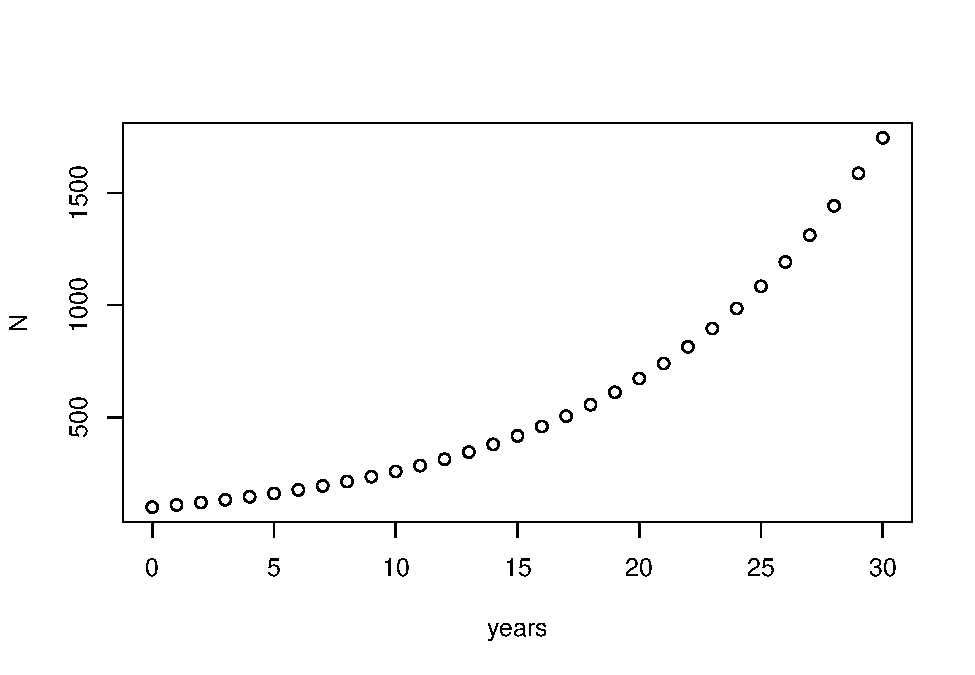
\includegraphics{LAB1_files/figure-latex/unnamed-chunk-7-1.pdf}

\hypertarget{exercise-2-r-related-problems}{%
\subsubsection{Exercise 2 (R-related
problems)}\label{exercise-2-r-related-problems}}

Please provide short answers to the following questions, and
\textbf{provide your R code to back up your answers}.

\begin{itemize}
\item
  \textbf{\emph{Short answer (2a.)}} Tweak the above code to run for 100
  years. Plot your results. What is the final population size?
\item
  \textbf{\emph{Short answer (2b.)}} Change r to 0.5 and run again for
  100 years (and plot the results). What is the final population size
  now? Include your plot as part of your answer.
\item
  \textbf{\emph{Short answer (2c.)}} Try to tweak the value of \(r\)
  such that the final population size after 100 years is 1000. What is
  the value of \(r\)? After you solve it by trial and error, can you
  solve this problem analytically using Eq. 10 above? Show your
  calculations!
\item
  \textbf{\emph{Short answer (2d.)}} Change the value of \(r\) to -0.1.
  How long until the population goes extinct? Explain your answer.
  Include a plot of your results.
\end{itemize}

\hypertarget{exponential-growth-in-insightmaker}{%
\subsection{Exponential growth in
InsightMaker}\label{exponential-growth-in-insightmaker}}

You should already have created a (free) account in
\href{https://insightmaker.com/}{insightmaker}, and you should already
know the basics about how to set up and run a model.

\begin{enumerate}
\def\labelenumi{\arabic{enumi}.}
\item
  Click ``Create New Insight'' to start a new model (click ``Clear this
  Demo'' to clear the canvas and have an open workspace). Save the blank
  model by clicking the ``Save'' button.
\item
  Create a new {[}Stock{]} named \emph{Population} using the
  ``\textbf{Add Primitive}'' button at top left (``Primitive'' is just a
  computer-sciencey term referring to basic building blocks of a
  computer programming language). You can name the {[}Stock{]} and
  configure it in the properties tab at the right.
\end{enumerate}

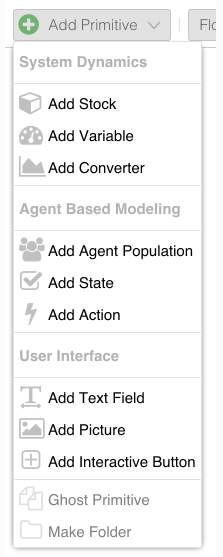
\includegraphics{IM1.png}

\begin{enumerate}
\def\labelenumi{\arabic{enumi}.}
\setcounter{enumi}{2}
\item
  Change the Initial Value of \emph{Population} to 100.
\item
  Create a new {[}Flow{]} going from empty space to the primitive
  \emph{Population} (make sure the \textbf{Flow/Transitions} button is
  activated instead of \textbf{Links} at the top, hover over
  \emph{Population} until an arrow appears, click and drag to create the
  {[}Flow{]}, use the \textbf{Reverse Connection Direction} button to
  change the flow direction). Name the flow \emph{Births}.
\item
  Create a new {[}Flow{]} going from \emph{Population} to empty space.
  Name the flow \emph{Deaths}.
\item
  The model diagram should now look something like this:
\end{enumerate}

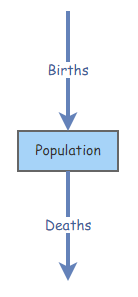
\includegraphics{IM2.png}

\begin{enumerate}
\def\labelenumi{\arabic{enumi}.}
\setcounter{enumi}{6}
\item
  Change the \textbf{Flow Rate} property of \emph{Births} to 0.16 \(*\)
  {[}Population{]}. This represents the total number of individuals
  entering {[}Population{]} in each time step.
\item
  Change the \textbf{Flow Rate} property of \emph{Deaths} to 0.10 \(*\)
  {[}Population{]}. This represents the total number of individuals
  leaving {[}Population{]} in each time step.
\end{enumerate}

Can you already tell whether this is a growing or declining population?
(just a quick thought question, not part of the written lab!)

\begin{enumerate}
\def\labelenumi{\arabic{enumi}.}
\setcounter{enumi}{8}
\tightlist
\item
  Run the model by clicking the \textbf{Simulate} button. We can change
  how the simulation is run by clicking the \textbf{Settings} button
  (left of Save). We can also change the settings of how the plot is
  created by clicking the \textbf{Configure} button within the
  simulation results window.
\end{enumerate}

\hypertarget{exercise-3-insightmaker-problems}{%
\subsubsection{Exercise 3 (InsightMaker
problems)}\label{exercise-3-insightmaker-problems}}

Please provide short answers to the following questions, and (when
prompted) \textbf{provide your ``Insights'' to back up your answers}.

First, tweak the above model so that per-capita (discrete) birth rate
(\(b_d\)) and death rate (\(d_d\)) are separate elements of the model
(using the ``Variable'' primitive). Your Insight should look something
like this:

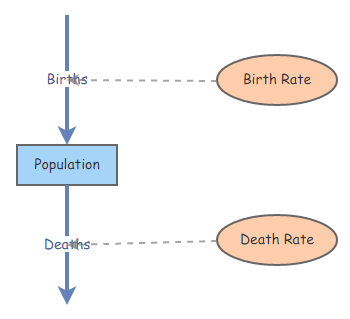
\includegraphics{IM3.png}

To enable easy manipulation of these variables, change the \textbf{Show
Value} Slider option of \emph{Birth Rate} (in the properties window) to
Yes. Change the \textbf{Slider Max value} to 1, the \textbf{Slider Min
value} to 0, and the \textbf{Slider Step value} to 0.01. Do the same for
\emph{Death Rate} and \emph{Population} (initial abundance \(N_0\)). For
abundance, set the maximum value to 1000 and set the slider step size to
1 so we don't have fractional individuals! Now click on the white space
of your model; you should now see the Birth Rate, Population and Death
Rate sliders on the info tab. Change the slider values of the rates a
few times, re-running the simulation each time. When you are confident
that your model is working right, share it with your instructor and TA
(save as a ``public insight'' and insert URL in the appropriate place in
Top Hat).

\textbf{Clone} your previous Insight before you move on to the next
problem (otherwise any changes you make will carry over to your answer
to the previous problem!). The ``Clone Insight'' link is located in the
upper right corner. In general, always clone your Insights after you
have copied a link to an insight into your lab write-up. That way, you
won't inadvertently change a model before your instructors have a chance
to verify you did everything right!

\begin{itemize}
\tightlist
\item
  \textbf{\emph{Short answer (3a.)}} Starting with a growing population,
  can you come up with two different scenarios in which
  \emph{Population} is neither growing nor declining, by only changing
  one of the sliders from the starting conditions? Explain your answer.
\end{itemize}

The simulations that you ran above produced population growth curves
that were very smooth, but we all know that populations don't grow in
this manner because of \textbf{stochasticity} (randomness). Let's add
some randomness to our vital rates! Change the \textbf{Show Value
Slider} option of the Birth Rate primitive to No.~Change the Equation to
0.1 + RandNormal(0, 0.1). The RandNormal() function generates a normally
distributed random number with \emph{mean (average) equal to the first
argument} and \emph{standard deviation equal to the second argument}.
This means that in each time step we have a slightly different birth
rate. Since we specified a \emph{mean} of zero, we are not actually
changing the average birth rate! Do the same for \emph{Death Rate}. Run
multiple simulations (at least 10) and look for patterns. Use the
\textbf{Compare Results} tool to compare and provide output. When you
are confident the model is right, add the URL for your InsightMaker
model to Top Hat in the appropriate place.

\begin{itemize}
\tightlist
\item
  \textbf{\emph{Short answer (3b.)}} Is it possible to have a declining
  population even when \emph{Birth Rate} and \emph{Death Rate} are the
  same? Is it possible to have a declining population when \emph{Birth
  Rate} is greater than \emph{Death Rate}? Explain your reasoning!
\end{itemize}

\#\#Checklist for Lab 1 completion *Please submit all files (Excel file,
and R code as text file) and responses via Top Hat. The InsightMaker
models should be shared by saving your Insights as ``public'' and
sharing the URL link with your instructors in Top Hat.

\textbf{\emph{Due Feb.~1}}

\begin{itemize}
\tightlist
\item
  Top Hat short answers

  \begin{itemize}
  \tightlist
  \item
    \textbf{Exercise 1}

    \begin{itemize}
    \tightlist
    \item
      \emph{Short answer (1a.)}
    \item
      \emph{Short answer (1b.)}
    \item
      \emph{Short answer (1c.)}
    \item
      \emph{Short answer (1d.)}
    \item
      \emph{Submit Excel file (1e.)}
    \end{itemize}
  \item
    \textbf{Exercise 2}

    \begin{itemize}
    \tightlist
    \item
      \emph{Short answer (2a.)}
    \item
      \emph{Short answer (2b.)}
    \item
      \emph{Short answer (2c.)}
    \item
      \emph{Short answer (2d.)}
    \end{itemize}
  \item
    \textbf{Exercise 3}

    \begin{itemize}
    \tightlist
    \item
      \emph{Short answer (3a.)}
    \item
      \emph{Short answer (3b.)}
    \end{itemize}
  \end{itemize}
\item
  Excel file (submit in Top Hat)

  \begin{itemize}
  \tightlist
  \item
    \textbf{Exercise 1}

    \begin{itemize}
    \tightlist
    \item
      Your Excel file should show that you were able to successfully use
      formulas to calculate \(N_t\) for each time step (year and month)
      and show a plot of \(N\) by Time.
    \end{itemize}
  \end{itemize}
\item
  R file (submit in Top Hat)

  \begin{itemize}
  \tightlist
  \item
    \textbf{Exercise 2}

    \begin{itemize}
    \item
      Your R code should show that you were able to (a) adapt the given
      code to run for 100 years, and can display a plot of the results;
    \item
      \begin{enumerate}
      \def\labelenumi{(\alph{enumi})}
      \setcounter{enumi}{1}
      \tightlist
      \item
        change \(r\) to 0.5 and run for 100 years and plot the results;
      \end{enumerate}
    \item
      \begin{enumerate}
      \def\labelenumi{(\alph{enumi})}
      \setcounter{enumi}{2}
      \tightlist
      \item
        identify a value of \(r\) that gives a population size of 1000
        after 100 years; and
      \end{enumerate}
    \item
      \begin{enumerate}
      \def\labelenumi{(\alph{enumi})}
      \setcounter{enumi}{3}
      \tightlist
      \item
        change \(r\) to -0.1 and run until the population goes extinct-
        and plot the results.
      \end{enumerate}
    \end{itemize}
  \end{itemize}
\item
  InsightMaker models

  \begin{itemize}
  \tightlist
  \item
    \textbf{Exercise 3}

    \begin{itemize}
    \item
      Your first model should show that you were able to alter the given
      model as instructed so that the simulation runs correctly. This
      should be shared via Top Hat (copy InsightMaker link in the
      appropriate place in Top Hat).
    \item
      Your second model should include stochasticity in \emph{Birth
      Rate} and \emph{Death Rate}. This should be shared via Top Hat.
    \end{itemize}
  \end{itemize}
\end{itemize}

\end{document}
